\subsubsection{Key Storage} \label{section:counter-replace-encryption-key-online}
Decryption needs a decryption key.
Since the encryption is only as strong as the protection of the key, this key has to be stored in a secure place.

\subsubsection{Key Storage - Online and Caching} \label{section:counter-replace-encryption-key-online}
The first approach to handle the encryption key is to store it on a server and provide it to the application.
This works similar to the license verification.
\newline
On decrypt method call, the application tries to retrieve a cached cryptographic key, which it has received and stored earlier.
In case a cached key is available, the application starts to decrypt the content.
Otherwise the key is requested from the server.
The server does a verification of the user and when the check is successful, the decryption key is send to the device instead of a guessable \textit{yes} or \textit{no}.
The advantage over the original implementation is that the key can neither be accessed without the verification on the server nor guessed by an attacker.
\newline
The key can either be retrieved from the server for each decryption action or it can be cached on the device, similar to the license verification policy.
Caching should be favored since getting the key for each action not only requires an online connection, but slows down the application and generates additional traffic.
\newline
In order to improve security, keys can be changed when updating the version of the application or be user specific.
\begin{figure}[h]
    \centering
    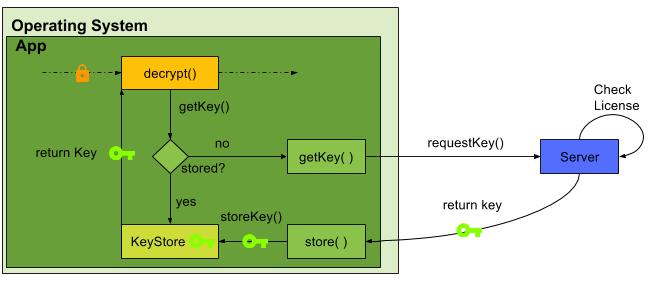
\includegraphics[width=1\textwidth]{data/encryptionKeyServer.png}
    \caption{Retrieving the key after successful identification from the server and store it local on device}
    \label{fig:encryptionKeyServer}
\end{figure}

\subsubsection{Key Storage - Secure Element} \label{section:counter-replace-encryption-key-local}
A cashed key can be stolen \cite{memoryDump} and the encryption cracked this way.
A \gls{se} can be used to prevent this.
\newline
A secure element is a tamper-resistant platform which can be used to securely host simple applications and cryptographic keys \cite{seDefinition}.
There are different form factors for \gls{se}s, i.e. Universal Integrated Circuit Card (UICC), embedded SE and microSD \cite{seDefinition}.
For Android, the microSD is the form factor of choice.
It can be either mounted in the microSD card slot or on the USB interface by using an adapter.
Using the USB interface requires the device to support \gls{otg} \cite{usbOtg}.
The \gls{se} is accessed over reads and writes to its filesystem.
Since the \gls{se} has to be small to fit the size of an microSD card and is powered by the host system, its hardware capabilities are constrained.
The result is a performance as low as 25MHz as compared to the GHz of the system's CPU.
This does not allow complex computations on the \gls{se}. \cite{stSe}
For this reason the usage of the \gls{se} is restricted to simple tasks, like storing a key used for decryption.
The advantage of an \gls{se} is that its functionality is outside of the Android application and thus cannot be manipulated by \gls{luckypatcherg}.
\newline
An abstract presentation for a \gls{se} that contains an applet to decrypt the input can be seen in figure~\ref{fig:encryptionKeySmart}.
\newline
\begin{figure}[h]
    \centering
    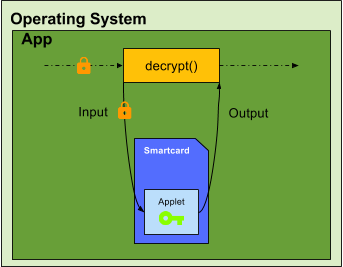
\includegraphics[width=0.5\textwidth]{data/encryptionKeySmart.png}
    \caption{Decryption by using a smartcard}
    \label{fig:encryptionKeySmart}
\end{figure}
At the moment, there are some problems with the integration of \gls{se}s.
\begin{itemize}
  \item the user has to buy extra hardware
  \item not all devices have a spare microSD card slot or support \gls{otg}
  \item no standardized communication protocols for the \gls{se} across manufacturers
\end{itemize}
The first problem is that the user has to buy extra hardware and the hardware has to be always around.
The second problem is the cable for devices without an microSD card slot since it is no convenient solution and is an easy target of an attack.
\newline
The third problem is that some devices without microSD card do not support \gls{otg}.
For example, the Nexus 7 (2012) and the Nexus 6P neither have the capability to use a microSD card.
While the Nexus 7 (2012) is supposed to have \gls{otg}, it does work with the a \gls{se}, while the Nexus 6P does not support \gls{otg} at all.
Both devices needed even additional plugins to read the \gls{otg} mounted microSD in a file explorer.
The third problem is the lack of standards.
An application written to use \gls{se} would need to have variants for each device type and manufacturer.
The SD Association has proposed a standard, if adopted the usage of \gls{se} might increase \cite{smartSD}.
